Numerous different groups have developed overlapping software for fast algorithms. For FMMs, leading analytical impelementations include the single-node multithreaded, `FMM3D' and `FMM2D' \cite{fmm3d, fmm2d}, and the MPI accelerated  `ExaFMM' \cite{exafmm} packages. The ExaFMM project have also developed a single-node multithreaded kernel-independent FMM, `ExaFMM-T' \cite{wang2021exafmm}. For algebraic methods, the landscape is sparser, with few parallel implementations. The standouts being the MPI accelerated `STRUMPACK' \cite{ghyselsstrumpack}, for HODLR and HSS matrices, as well as the multithreaded single-node `FLAM' \cite{ho2020flam}, which supports algorithms for $\mathcal{H}^2$ matrices. The majority of codes, except FLAM, are written in either Fortran or C++, with a few supporting interfaces to higher level languages such as Python and Matlab \cite{wang2021exafmm,fmm3d}.

We compare these softwares for the calculation of (\ref{eq:two_box_calc:sec_1_2}) with $N$ randomly distributed particles placed in a unit cube, $[0, 1]^3$, with uniform charge, $q_i=1$, in figure (\ref{fig:sec_2_0:software_comparison}) \footnote{Our experiments are available at \url{https://github.com/skailasa/phd-thesis/code/ch_2/}}. Experiments are taken on a single-node AMD Ryzen Threadripper 3970X 32 core Processor, with 250GB of memory. To avoid thread oversubscription in STRUMPACK and ExaFMM, both designed for multi-node systems, the maximum number of OpenMP threads is restricted to one. Each FMM software is run with an expansion order $P=10$, and the algebraic software's parameters are adjusted to match this level of accuracy.

In comparing these softwares we aimed to emulate the workflow of a typical user evaluating the differences between software packages, and therefore restricted our study to runs which converged in less than 30 minutes, $\approx 2 \times 10^3$ s. Figure (\ref{fig:sec_2_0:software_comparison}a) plots the time to compute (\ref{eq:two_box_calc:sec_1_2}), including the time to create all required data structures. For the algebraic softwares, FLAM and STRUMPACK, this includes the time to factorise and store an explicit matrix representation of (\ref{eq:two_box_calc:sec_1_2}). Strictly speaking, STRUMPACK's HSS and HODLR matrices are not applicable to (\ref{eq:two_box_calc:sec_1_2}), as it is a strongly admissable problem. We see the effects of this in super-quadratic factorisation times for increasing $N$. Additionally, FLAM, written in Matlab, is not designed for high performance. However, these remain the only well supported, publicly available, parallel implementations of algebraic fast algorithms and we include them for comparison. As expected, the factorization scales super-linearly for both softwares, which lies in contrast with their relatively fast matrix vector products once factorised (fig. (\ref{fig:sec_2_0:software_comparison}c)). 

We observe that currently available open source algebraic software is impractical for computing even moderately sized matrix vector products, i.e. $N \geq O(10^5)$. With runtimes times for factorisation exceeding our imposed limit of $2 \times 10^3$ s. One might argue that their expensive factorization cost is worth it if one proceeds to compute (\ref{eq:two_box_calc:sec_1_2}) multiple times, or if one wants to quickly find an inverse. However, the FMM softwares tested beat both algebraic softwares by several orders of magnitude, making it much more tenable to apply them multiple times if required, and to find matrix inverses via an iterative Krylov type methods.

\begin{figure}
    \begin{tabular}{cc}
        \subfloat[\centering Runtime]{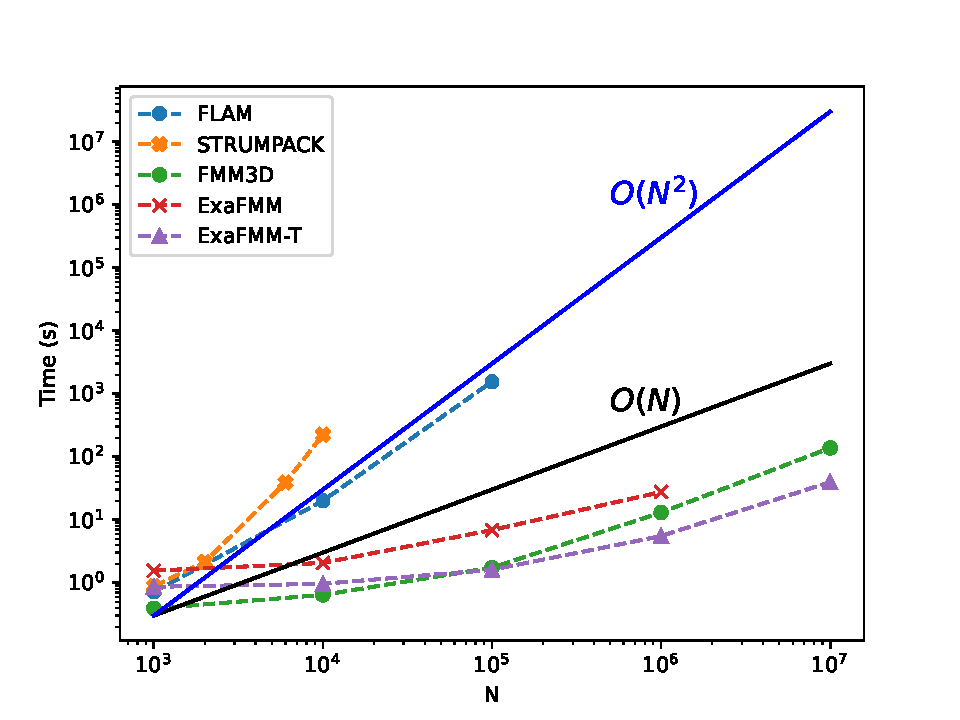
\includegraphics[width=75mm]{ch_2/runtime.pdf}} & \subfloat[\centering Peak memory]{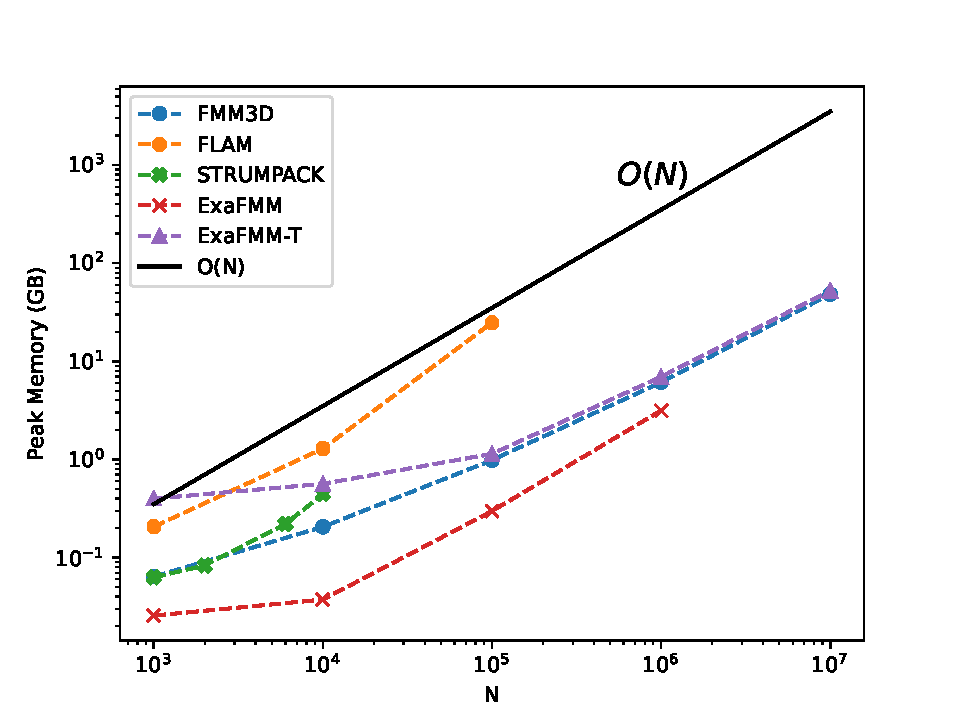
\includegraphics[width=75mm]{ch_2/memory.pdf}}
    \end{tabular}
    \centering \subfloat[\centering Matrix vector product time for algebraic methods.]{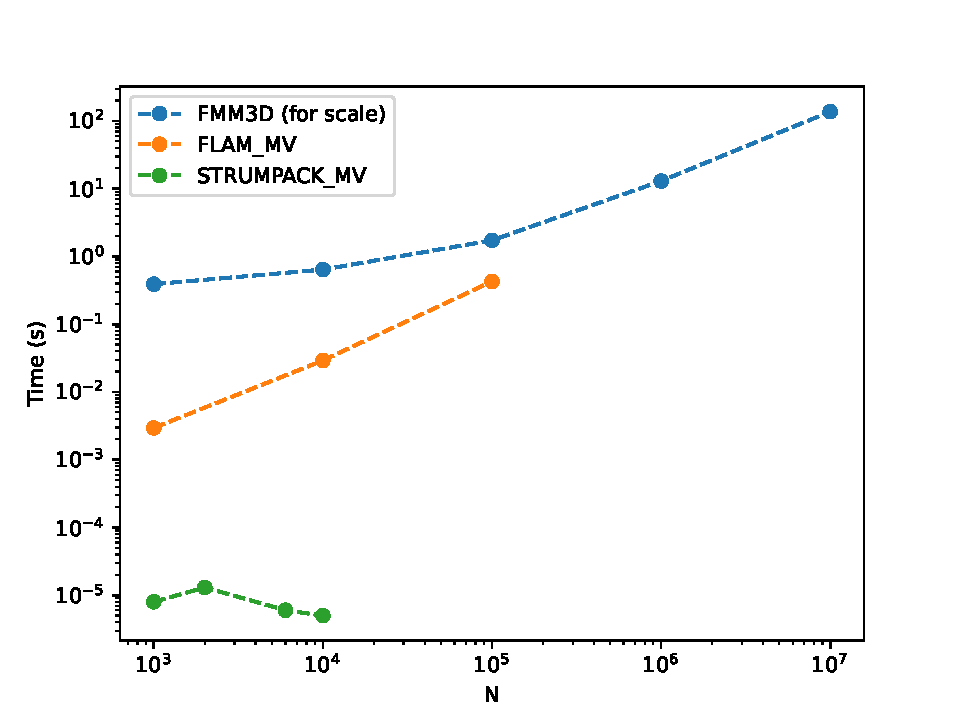
\includegraphics[width=75mm]{ch_2/alg_matvec.pdf}}
    \caption{Comparison of parallel software for fast algorithms, used to caclulate (\ref{eq:two_box_calc:sec_1_2}). Simulations were compared for convergence times $\leq 2 \times 10^3$ s that could fit into memory.}
    \label{fig:sec_2_0:software_comparison}%
\end{figure}

As expected from theory, the analytical FMMs, ExaFMM and FMM3D, consume less memory than the kernel-independent ExaFMM-T (fig. (\ref{fig:sec_2_0:software_comparison}b)). However, for larger problem sizes this difference is marginal between FMM3D and ExaFMM-T. For the largest problem size tested, $N=10^7$, ExaFMM-T is roughly 3.5 times faster than FMM3D with a similar memory footprint. Counter intuitively, the analytical ExaFMM fails to converge in our experiments for $N=10^7$, as its memory requirements exceed the available 250 GB. 

Theoretical considerations aside, each software's performance is practically determined by the computational and algorithmic performance optimisations they take. ExaFMM-T for example uses optimized algorithms for the calculation of inverse square roots \cite{malhotra2015pvfmm}, as well as using SIMD vectorisation for kernel evaluations \cite{wang2021exafmm}. Similarly by stacking $T^{M2L}$ as in (\ref{eq:sec_1_2:m2l_stacked}), they optimise cache-reuse. Similar SIMD vectorisations are implemented by FMM3D and ExaFMM, however their remaining optimisations are presented opaquely, making it difficult for users to evaluate their relative merits.

Usability, defined in terms of quality of API documentation, available descriptions of mathematical and software optimisations,  quality of software engineering in terms of self-documenting and well commented code, as well as ease of installation, is as critical to the dissemination of scientific software as raw performance. It's unlikely that a user will incorporate a performant piece of software into their work if it's not usable. In this respect FMM3D and ExaFMM-T standout, with well documented APIs, code examples, as well as wrappers to call functionality from higher level languages. STRUMPACK, though relatively well documented, does not support wrappers to higher-level languages. Written in C++, its documentation is largely a description of its object hierarchy, with few examples documenting real world use cases. ExaFMM on the other hand is poorly documented, with few tests or comments, and no wrappers to high-level languages. Most softwares, except STRUMPACK which is distributed via the SPACK package manager, have traditional source builds based on CMake and Make. Local installation can therefore be challenging when building on non-traditional HPC operating systems such as Windows and MacOS.

From the experiments in figure (\ref{fig:sec_2_0:software_comparison}) it's clear that software choice can have dramatic impact on runtime and memory scaling regardless of algorithmic choice. For the Laplace problem of (\ref{eq:two_box_calc:sec_1_2}) all softwares can be used more or less out of the box, however oscillatory Helmholtz kernels are only natively supported by a few \cite{exafmm,wang2021exafmm,fmm2d, fmm3d}. The most complete functionality, with the addition of Stokes and Maxwell kernels, are only supported by FMM2D and FMM3D. From a non-expert user's perspective, merely understanding the theory behind each algorithm isn't enough to expect a guaranteed performance, as demonstrated by the poor scaling of algebraic softwares, as well as the different memory requirements of the analytical FMMs. In light of this, users would likely be tempted to pick a `median' option, which guarantees good performance, scalability, easy installation, and usability via a high-level language wrapper and support for multiple problems. This makes FMM2D and FMM3D the standout options, however as they're developed as a high-performance Fortran libraries, they are relatively unmalleable, with a steep learning curve for potential contributors and limited to single-node systems.

In conclusion, we identify a distinct lack of software for fast algorithms that fulfills our usability criteria and can also scale to multi-node systems. Presently available software is not composable, with differing APIs and re-implementations of high-performance kernels as well as data structures such as quad and octrees. Algebraic methods lack an optimised software for strongly admissable problems, with FLAM designed as a research code for prototyping purposes. Wrappers for high-level languages are not uniformly available, and builds can be challenging in non-Linux environments.

We aim to solve this with our proposed software infrastructure (fig (\ref{fig:sec_2_0:rusty_roadmap})). By offering a set of composable libraries with a unified API for FMMs and algebraic methods for constructing matrix inverses, we aim to maximally re-use highly-optimised code, such as for SIMD vectorised kernel evaluations, and quad and octrees that can scale across multiple processors. We propose Rust as the language for our this infrastructure. We initially explored high-performance code generation tools for Python as a bridge between an ergonomic language for researchers and developers with high-performance. This is documented in chapter \ref{chpt:3} via our attempt to build a Python FMM. Due to the constraints of development in high-level languages, and not wishing to use C/C++ or Fortran, we pivoted to Rust. Rust is a young low-level systems programming language, with significant industry support, which has many features that improve the usability of scientific software. Most importantly its build system, Cargo, is specified by a simple TOML file, making it easy to deploy Rust codes on most common platforms without the need for complex build CMake style build scripts. This will make it easy for users to develop software locally, before deploying to a super computing cluster, while still being able to expect good performance. Rust's syntax inherits from both functional and imperative paradigms, and its trait system wholly replaces object orientation, making the description of shared behaviour, and data oriented programming, significantly more readable. However, importantly, it is also easy to develop wrappers from Rust to Python using its C foreign function interface \cite{maturin2022github}, allowing us to expose our infrastructure to novice programmers. We document the prominent features of Rust that make it useful for scientific computing in chapter \ref{chpt:4}, before exploring the performance of a completed Rust based library for MPI accelerated octrees in chapter \ref{chpt:5}.

\begin{figure}
    \centerline{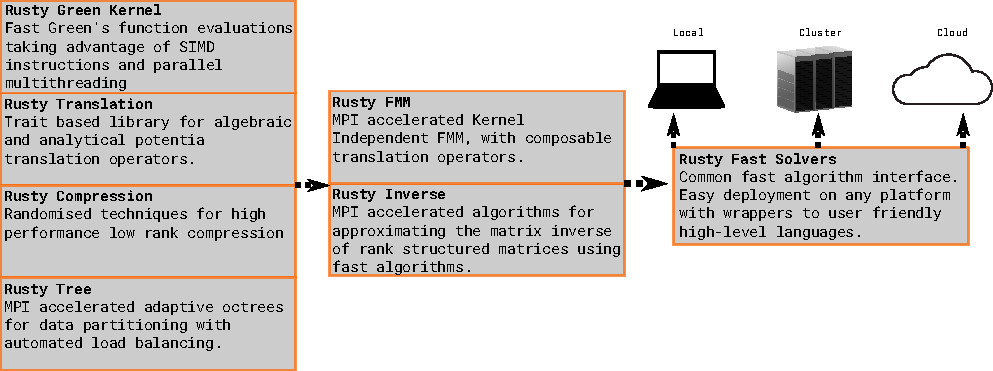
\includegraphics {ch_2/rusty_roadmap.pdf}}
    \caption{Hierarchy of our proposed infrastructure, with key functionality separated into individual libraries we maximise code re-use across projects. Once completed using Rust's code generation infrastructure, users will be able to deploy our software from desktop workstations, to supercomputing clusters and expect scalable high-performance code, while being able to write application code in Python.}
    \label{fig:sec_2_0:rusty_roadmap}
\end{figure}
